% !TEX root = ../../../main.tex
% 来源：中学数学实验教材·第二册（几何）
% 章节：实验几何 / 方向、角度与平行
% 原始文件：1.tex，行 1377-1391
% 类型：tikz
% ---
	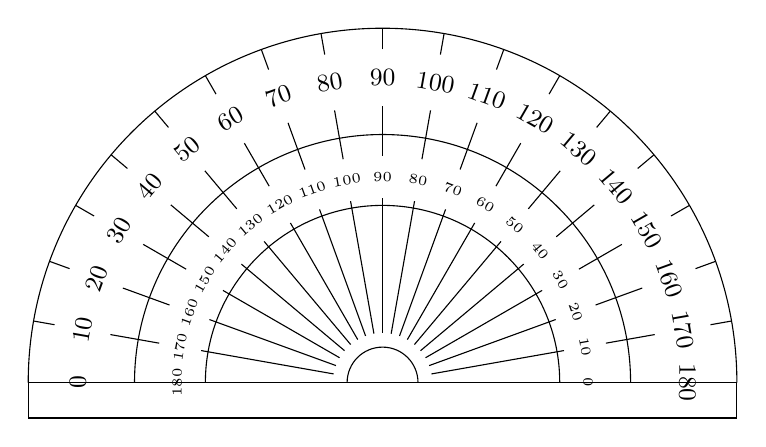
\begin{tikzpicture}[scale=.9]
\draw(-5,0) rectangle (5,-.5);	
\foreach \x in {.5, 2.5,3.5,5}
{
	\draw(\x ,0) arc (0:180:\x );
}
\foreach \x in {0, 10,20,...,170,180}
{
	\draw (\x:0.7)--(\x:2.6);
	\draw (\x:3.2)--(\x:3.9);
	\draw (\x:4.7)--(\x:5);
	\node[rotate=-90+\x] at (\x:2.9){\tiny \x};
	\node[rotate=90-\x] at (180-\x:4.3){\small \x};
}
\end{tikzpicture}
